\chapter{Background and Preliminaries} \label{ch:Intro}

\section{Optical- and Photonic Crystal- Fibres} \label{sec:PCFs}
Optical fibres are the \textit{de facto} industry standard for large telecommunications systems, thanks to their ability to transmit information quickly and with far less signal loss than other methods (such as metal cables).
The technology has rapidly developed since the first optical fibres were fabricated in the 1970s \cite{knight2003photonic} and optical fibres in use today present a balance between several competing factors to deliver a reliable performance.
Factors such as (optical) loss are inherent, brought about by the materials needed to build the fibres; whilst other factors can be influenced by design (group-velocity dispersion) or the fabrication process (which can lead to imperfections and polarisation effects).
Despite the technological developments of the fibres, the underpinning physical processes remain unchanged --- all improvements to the technology have been incremental and largely centre around the manufacturing process.
The fibre will have a core made of a dielectric (non-conducting) material with a given refractive index, $\rInd{core}$ and will be surrounded by cladding, another dielectric material of a different index $\rInd{cladding}$ (\fref{OpticalFibre}).
\begin{figure} [b!]
	\centering
    \subfigure[Cross-sectional design of an optical fibre, which uses TIR to guide light. Modes are restricted to the core by the choice of $k_{p}$ and as $\rInd{core}>\rInd{cladding}$. \label{fig:OpticalFibre}]{
        \centering
        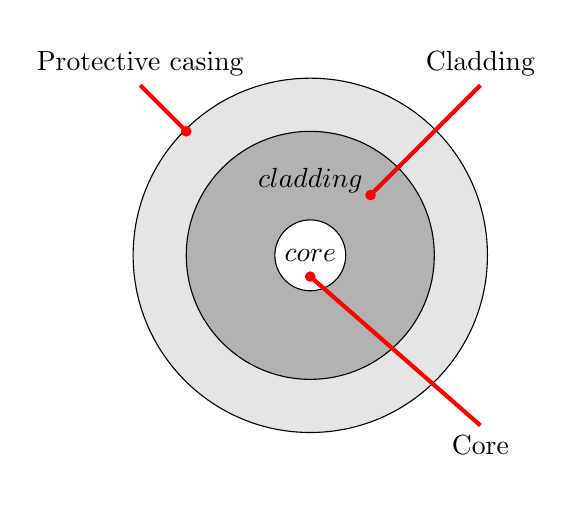
\begin{tikzpicture}
        	\begin{scope}[scale=0.9]
	        	\filldraw[fill=black!10!white, draw=black] (0,0) circle (2.5);       	
	        	\filldraw[fill=black!30!white, draw=black] (0,0) circle (1.75);
	        	\filldraw[fill=black!0!white, draw=black] (0,0) circle (0.5);
	        	\draw[line width=1.5, color=red] (-1.75,1.75) -- (-2.4,2.4);
				\node[anchor=south] at (-2.4,2.4) {Protective casing};
				\fill[color=red] (-1.75,1.75) circle (0.075);
	        	\draw[line width=1.5, color=red] (0.85, 0.85) -- (2.4,2.4);
				\node[anchor=south, align=center] at (2.4,2.4) { \\ Cladding}; %life hacks, makes diagrams aligned nicely (don't remove \\!)
				\fill[color=red] (0.85,0.85) circle (0.075);
	        	\draw[line width=1.5, color=red] (0,-0.3) -- (2.4,-2.4);
				\node[anchor=north, align=center] at (2.4,-2.4) {Core \\};
				\fill[color=red] (0,-0.3) circle (0.075);
				\node at (0,0) {$\rInd{core}$};
				\node[anchor=south] at (0,0.75) {$\rInd{cladding}$};
			\end{scope}
        \end{tikzpicture}
	}
	\quad
	%\enspace
    \subfigure[Cross-section of a PCF which uses the existence of photonic band gaps to confine light. The photonic crystal is represented by the black hexagons whilst the solid/hollow cores are the white fillings. \label{fig:PCFDiagram}]{
        \centering
		\begin{tikzpicture}
			\begin{scope}[scale=0.9]
				\filldraw[fill=black!10!white, draw=black] (0,0) circle (2.5);
				\draw[line width=1.5, color=red] (-1.75,1.75) -- (-2.4,2.4);
				\node[anchor=south] at (-2.4,2.4) {Protective casing};
				\fill[color=red] (-1.75,1.75) circle (0.075); %casing and label
				\filldraw[fill=white, draw=black] (0,0) circle (1.75);
				\filldraw[pattern=hexagons, draw=black] (0,0) circle (1.75); %hexagons
				\draw[line width=1.5, color=red] (0.8,1.0) -- (2.4,2.4);
				\fill[color=red] (0.8, 1.0) circle (0.075);
				\node[anchor=south, align=center] at (2.4,2.4) {Photonic Crystal \\ (black lines)};
				\node[anchor=north, align=center] at (2.4,-2.4) {Solid or hollow \say{cores} \\ (white space)};
				\draw[line width=1.5, color=red] (0.9,-1.0) -- (2.4,-2.4);
				\fill[color=red] (0.9, -1.0) circle (0.075);
				%core circle
				\filldraw[color=white] (0,0) circle (0.75);
				\draw[color=black] (0,0) circle (0.75);
			\end{scope}
		\end{tikzpicture}
	}
	%general caption
	\caption{Difference in the cross-sectional structure of an optical fibre and a PCF. The optical fibre will guide modes within a given modal (index) range. The PCF microstructure vary, and certain structures can be engineered to confine different frequencies of light. \label{fig:FibreComparison}}
\end{figure}
The fibre then relies on total internal refraction (TIR) to guide light along the fibre.
When a light ray in the core strikes the core-cladding boundary Snell's law determines the angle at which the light ray propagates upon entering the cladding\footnote{The \say{deflection} of the ray as it passes between the materials is the well-known phenomenon of refraction.},
\begin{align} \label{eq:SnellsLaw}
	 \rInd{core}\sin\ang{i} &= \rInd{cladding}\sin\ang{t};
\end{align}
where $\ang{i}$ and $\ang{t}$ are (respectively) the angles of incidence and transmission from the boundary.
It's possible for $\ang{t}>\frac{\pi}{2}$ provided that $\rInd{core}>\rInd{cladding}$; in which case (TIR happens and) the light ray does not enter the cladding at a refracted angle, but rather is totally reflected and continues propagating through the core.
Equation \eref{SnellsLaw} can also be used to show that the component of the wavevector parallel to the core-cladding interface, $k_{p} = \rInd{core}k\sin\bracs{\ang{i}}$, remains unchanged during the interaction and so is constant along the fibre for a given mode\footnote{A mode is a single solution to the wave equation in the fibre.}.
For any given material with refractive index $N$, all values $k_{p}\leq Nk$ allow light to propagate in the medium\footnote{This is an upper bound as it's derived by looking at an infinite, homogeneous \say{slab} of the material.}, and for each $k_{p}$ the modal index is defined as $\rInd{m} = \frac{k_{p}}{k}$.
To form a guided mode light must have a value of $k_{p}$ which cannot propagate in the cladding but which can propagate in the core, which can be satisfied by ensuring that
\begin{align*}
	&\rInd{cladding}k \leq k_{p} \leq \rInd{core}k \\
	\Leftrightarrow &\rInd{cladding} \leq \rInd{m} \leq \rInd{core} .
\end{align*}

Photonic crystals can be used as cladding for a conventional fibre; these crystals also have a maximal value of $k_{p}$ which allows light to propagate in them, and this maximal value defines an \say{effective refractive index} in accordance with $\rInd{eff} = \frac{k_{p}}{k}$.
Therefore, if at a particular frequency (equivalently $k$, however it is conventional to work with the frequency here) $\rInd{eff}<\rInd{core}$, the photonic crystal can be used as cladding material and will guide light via a form of TIR. 
Photonic crystal \textit{fibres} (PCFs) are a departure from the setup of core surrounded by cladding \cite{russell2003photonic}; instead relying on the microstructure of the photonic crystal to alter the optical properties of the fibre it forms.
This microstructure can cause the crystal to exhibit band-gaps; frequency ranges\footnote{Respectively $k$-ranges or $N_{m}$ ranges, \cite{knight2003photonic}, \cite{russell2003photonic}.} where there are no propagating modes of light in the crystal, despite the existence of propagating modes at lower (and/or higher) frequencies.
The important revelation comes in the fact that band-gaps can appear for frequencies corresponding to $\rInd{eff}<1$, which means that light in vacuum at these frequencies will be confined if surrounded by such a crystal - making \say{hollow-core} fibres possible.
The term hollow-core refers to a PCF with vacuum as its \say{core material}, PCFs can also be \say{solid-core} with another material in them (\fref{PCFDiagram}).
Crucially though, these fibres do not use TIR to guide light but rather exploit the fact that light at particular frequencies is confined simply because it is unable to propagate in the surrounding crystal, due to the optical properties bestowed on the crystal by its microstructure.
\Fref{FibreComparison} illustrates the difference in fibre design between optical fibres and PCFs. \newline

PCFs have been the subject of a number of mathematical models in recent years.
The standard starting point for these models is the time-harmonic system of Maxwell equations
\begin{align*}
	\grad\wedge\mathbf{E} &= i\omega\magP\mathbf{H}, &\quad \grad\wedge\mathbf{H} &= -i\omega\elcP,\mathbf{E}
\end{align*} 
where $\mathbf{E}$ and $\mathbf{H}$ are the electric and magnetic (-displacement) fields respectively, and the medium in which the problem is posed has electric permittivity $\elcP$\footnote{The subscript being used to distinguish the microstructure length scale $\epsilon$ (which will be introduced later) and electric permittivity in the event of confusion.} and magnetic permeability $\magP$. 
Note that the reason for using the time-harmonic Maxwell system arises from consideration of the fibre structure\footnote{That is, as a 2-dimensional periodic structure extended into three dimensions as a prism.} and seeking solutions via a wave ansatz of the form $\hat{\mathbf{E}}=\mathbf{E}e^{i\bracs{k_{p}z-\omega t}}$ (and similarly for the magnetic field); these are referred to as Bloch waves.
Further assumptions are also made on the fields, namely that the amplitude coefficients $\mathbf{E},\mathbf{H}$ are functions of $x,y$ only, and do not vary along the fibre.
This assumption is well-grounded as these models are seeking waves that will propagate down the fibre, and expect the $\mathbf{E}$ and $\mathbf{H}$ fields to vary only in the plane perpendicular to the direction of propagation.
As for the domain of the problem which describes the microstructure and hence the fibre, models assume a unit cell (commonly taken to be the unit square) and periodically extend the domain from this.
The unit cell itself is taken to be composed of two materials with different material constants, which means $\elcP$ and $\magP$ become piecewise-constant functions of the $(x,y)$ variables.
This provides a general model for any kind of periodic structure, rather than the specific geometry we will restrict ourselves to in future.
Analysis of this model and the solution properties can be found in (for example) \cite{cooper2014bandgaps} and \cite{soussi2006modeling}.
The approach is to apply homogenisation theory due to the periodic structure of the domain, and introduce  an appropriate representation of a periodic problem on the unit cell.
One can then prove convergence results for various aspects of the unit-cell problem and the original periodic problem (most notably the spectrum of the problem, which determines the frequencies $\omega$ of light which can propagate).
The work in \cite{soussi2006modeling} makes a few more assumptions on the model and produces results relating to the decay of certain solutions as well.
When the task is to find solutions to the Maxwell system, one often turns to numerical schemes to produce approximations for visualisation.
The use of the time-harmonic Maxwell equations means that methods such as the Finite Element Method can be used, and there is no need to incorporate time-variation into the numerical scheme, which is a bonus in terms of computation time and algorithm complexity. \newline

In summary, PCFs present a \say{cautiously optimistic} improvement to the current industry standard.
The physical theory underlying the process by which they operate means that PCFs have the potential to replace optical fibres as the industry standard.
This is not a simple case of fabricating better fibres, but rather there are several industry standards that will need to be met before PCFs are accepted and implimented over optical fibres \cite{knight2003photonic}.
However PCFs have an advantage over optical fibres in that their applications are not only limited to telecommunications.
At present prominant aternative applications include (but are not limited to) nonlinear optics (where they offer high optical intensities per unit power, making them highly efficient) and atom and particle guidance (dielectric particles can be guided by the dipole forces exerted by light).
Hence there has been much to motivate study of the optical properties of PCFs, and understand how the design (geometry of the fibre, fabrication material) affects these, resulting in the models based on the Maxwell equations and development of spectral convergence results for periodic problems.

\section{Singular Structure Problems} \label{sec:GraphPrelims}
We will be looking to analyse problems posed on singular structures (to motivate the discussion in \cref{WorkDirection}) and so present some theory that will justify the methods we use.
We restrict ourselves to cases that are directly applicable to the analysis we are looking to perform, and so focus on graphs embedded in Euclidean space $\reals^{d}$, and which exhibit periodic structure in each dimension. 
The theory extends beyond this \cite{kuchment2013introduction}, being applicable in much more general settings and with graphs that have other complicating factors.
These more general problems are sometimes referred to as \say{quantum graphs}. \newline

Let $\graph = (V,E)$ be a graph with set of vertices $V$ and edges $E$.
Suppose further that $\graph$ is embedded in $\reals^{d}$; namely that each $v_{i}\in V$ can be associated with a point $\mathbf{v}_{i}\in\reals^{d}$ and each $e_{ij}=\bracs{v_{i},v_{j}}\in E$ can be identified with the line segment joining $\mathbf{v}_{i}$ and $\mathbf{v}_{j}$.
With this identification of vertices and edges we can use subsets of $\reals^{d}$ to describe subgraphs of $\graph$, and vice-versa.
If $U\subset\reals^{d}$ (for example), then the \say{part of $\graph$ in $U$} is the subgraph which consists of all vertices whose associated point lies in $U$, and all edges between those points whose associated line segment lies entirely in $U$.
Concepts such as translations and rotations of the graph can also be understood as being applied to the associated points and segments in $\reals^{d}$.
We also impose some periodic structure on $\graph$; which is to say that there exists some finite subset $\mathcal{U}\subset\reals^{d}$ and corresponding subgraph $\graph_{\mathcal{U}}$ such that $\graph$ is a (possibly infinite) union of translations of $\graph_{\mathcal{U}}$.
Colloquially, $\graph$ can be assembled by stacking (in each of the $d$-dimensions) copies of the graph $\graph_{\mathcal{U}}$. 
We use the term \say{\textit{unit cell} of $\graph$} to refer to this subset $\mathcal{U}$ or subgraph $\graph_{\mathcal{U}}$. 
Without loss of generality we take the unit cell of $\graph$ to be a (hyper-) cube of side length $l$. \newline

We denote the space of complex-valued square-integrable functions on $\graph$ by $\lp{2}{\graph}$.
Identifying each edge $e_{ij}$ with some one-dimensional interval $I_{ij}\subset\reals$, any $u\in\lp{2}{\graph}$ can be identified with a set of \say{edge}-functions $\mathset{u_{ij}:I_{ij}\rightarrow\compx}$.
Next, we let $\graphOp$ be an operator defined on functions $u\in \lp{2}{\graph}$; of the form $\graphOp u = -\grad\cdot\bracs{A\grad u}$, and whose spectrum we wish to obtain.
This requires solving the eigenvalue-eigenfunction equation
\begin{align*}
	-\grad\cdot\bracs{A\grad u} &= \omega^{2}u
\end{align*}
for $\omega\in\reals$ and\footnote{The operator $\graphOp$ is self-adjoint, and hence has a real spectrum. The choice of $\omega^{2}$ (presupposing an entirely real spectrum) is posthumously justified in later sections.} $u\in\lp{2}{\graph}$.
Solutions are found by solving 
\begin{align*}
-\diff{x}\bracs{a_{ij}\diff{x}u}=\omega^{2}u
\end{align*} 
on each of the intervals $I_{ij}$ (also described as solving \say{on the edges $e_{ij}$}), and appropriate matching conditions at the vertices, to give $u\in\lp{2}{\graph}$ in terms of it's edge components.
Here $a_{ij}$ is just the appropriate restriction of $A$ to the edge $e_{ij}$.
For periodic graphs it is customary to apply a Gelfand transform to $\graphOp$ to aid in analysis of these problems, which provides a way of representing the operator $\graphOp$ in terms of a family of operators $\graphOp^{\Theta}$.
Here $\Theta=\bracs{\tho, \tht, ..., \theta_{d}}$ is a parameter of the family of operators $\graphOp^{\Theta}$ that we need to study, and the $\theta_{i}$ are the quasi-momenta (one for each periodic direction of the graph) which range over\footnote{The quasi-momenta have a range determined by the size of the period cell in each dimension. As we assume a (hyper-) cube period cell, each quasi-momentum has the same range. For more general unit cells, different quasi-momentum will have different ranges.} $[-\frac{\pi}{l},\frac{\pi}{l})$.
The Gelfand transform then represents $\graphOp$ as a direct integral of the operators $\graphOp^{\Theta}$ over the quasi-momenta\footnote{The Gelfand transform can be seen as a generalisation of the familiar Fourier transform. Indeed, the Fourier transform \textit{is} the Gelfand transform in a specific context.}.
Importantly, the Gelfand transform means that determining the spectrum of $\graphOp$ can be done by determining the spectrum of $\graphOp^{\Theta}$ and taking the union over all $\tho, \tht, ..., \theta_{d}$. 
It is this fact which we shall make use of in the analysis of the following problems. \newline

It should be noted that several assumptions and simplifications have been made in the above discussion, the details of which will not be elaborated on.
The foremost of these is the construction of the Hilbert space $\lp{2}{\graph}$, and the fact that the Gelfand transform has to be extended by $L^{2}$-closure to be applicable to (operators on) non-smooth functions.
Furthermore, when applying the Gelfand transform to graphs embedded in $\reals^{d}$ we have assumed the graph is periodic in all $d$-directions, however in general the graph may be periodic in $d'<d$ directions.
For a graph periodic in one direction and with a finite periodic cell, an auxiliary procedure called \say{flattening} can be applied to the graph before the Gelfand transform, to reduce the complexity of the setup.
An example of (and a description of the flattening proceedure) a graph embedded in $\reals^{d}$ but only periodic in only one dimension can be found in \cite{ershova2018gelfand}.

\section{Discussion of Length and Frequency Scalings} \label{sec:FreqApproxes}
Besides singular structure problems we will also consider problems posed on thin-structure periodic domains in $\reals^{d}$.
Denote such a domain by $\homDomain$; which similarly to the periodic graphs is composed of translations of a unit cell, but which (unlike the singular-structure problems) possess microstructure on a different length scale to the unit cell.
We assume (without loss of generality) that the period cell is a (hyper-) cube with side length 1, with microstructure of length scale $\epsilon$, denoted by $P_{\epsilon}$. 
In this section we aim to briefly introduce the various frequency frameworks that exist for problems of this kind, and how they are interlinked.
Analogously to \sref{GraphPrelims} we are interested in the spectrum of the operator $\graphOp u = -\grad\cdot\bracs{A\grad u}$ for $u\in\lp{2}{\homDomain}$ and so examine the eigenvalue-eigenfunction equation 
\begin{align} \label{eq:AsymExample}
	-\grad\cdot\bracs{A\grad u} = \omega^{2}u.
\end{align}
The expressions $P_{\epsilon} + \vx$ for $\vx\in\reals^{3}$ are interpreted as the translation of all points in the unit cell $P_{\epsilon}$ by the vector $\vx$, and $\alpha P_{\epsilon}$ as the scaling of the unit cell $P_{\epsilon}$ by the scalar $\alpha$.
To setup the finite-frequency approximation we introduce the domain length scale $N$, which for simplicity we shall take to be a multiple of the side-length of our periodic unit cell (so $N\in\naturals$).
Next we construct another (related) problem on a finite domain $\homDomain_{F}$; which we construct by stacking $N^{d}$ copies of $P_{\epsilon}$, with $N$ stacked along each axis so that
\begin{align*}
	\homDomain_{F} =\bigcup_{x,y,z\in\{0,1,...,N\}}\bracs{P_{\epsilon} + \bracs{x,y,z}^{\top}}\subset [0,N]^{3}.
\end{align*}
At the boundary of $\homDomain_{F}$ we impose periodic boundary conditions; these effectively mimic the fact that $\homDomain$ fills the whole of $\reals^{d}$ with some periodic structure, and our finite-frequency approximation is looking for solutions which are periodic across $N$ unit cells.
with periodic boundary conditions imposed on $\partial\homDomain_{F}$.
We still seek solutions to \eref{AsymExample} on $\homDomain_{F}$, only now $u\in\lp{2}{\homDomain_{F}}$.
Hence in the finite-frequency approximation we are looking to find the spectrum of the operator $\graphOp_{N}$, defined on functions $u\in\lp{2}{\homDomain_{F}}$.
Passing to the limit $N\rightarrow\infty$ results in the spectrum of the operators $\graphOp_{N}$ converging to the spectrum of the operator in the full space ($\graphOp$). \newline

Having established a finite-frequency approximation it makes sense to talk about alternative frequency approximations.
One can think of a high-frequency approximation to the original problem; which is posed on a (hyper-) cubic domain of side length 1, but composed of $N^{d}$ copies of $\recip{N}P_{\epsilon}$ (stacked).
This domain,
\begin{align*}
	\homDomain_{H} = \recip{N}\homDomain_{F} = \bigcup_{x,y,z\in\{0,\recip{N},...,1\}}\bracs{\recip{N}P_{\epsilon} + \bracs{x,y,z}^{\top}} \subset [0,1]^{3},
\end{align*}
again has periodic boundary conditions on $\partial\homDomain_{H}$, and again we obtain a sequence of operators (parametrised by $N$) and their corresponding spectra.
In the limit $N\rightarrow\infty$ this gives us the spectrum of an operator on a finite, homogenised domain.
Additionally we can move between the high- and finite-frequency approximations using a domain-length-scale (and complimentary frequency-scale) change: in the high-frequency regime we have the problem
\begin{align} \label{eq:HFEqn}
	-\grad\cdot\bracs{A\bracs{\vx}\grad u\bracs{\vx}} &= \omega^{2}u\bracs{\vx}, \quad \vx\in\homDomain_{H},
\end{align}
and rescaling the domain-length-scale via $\vy = N\vx$, \eref{HFEqn} becomes
\begin{align}
	&-\recip{N}\grad_{\vy}\cdot\bracs{A\bracs{\vy}\recip{N}\grad_{\vy} u\bracs{\vy}} = \omega^{2}u\bracs{\vy}, &\quad \vy\in \homDomain_{F} \\
	\Leftrightarrow
	&-\grad_{\vy}\cdot\bracs{A\bracs{\vy}\grad_{\vy} u\bracs{\vy}} = \bracs{N\omega}^{2}u\bracs{\vy}, &\quad \vy\in\homDomain_{F},
\end{align}
which implies that the accompanying frequency scaling $\omega\rightarrow N\omega$ can be used to understand the spectrum in one frequency approximation, given the spectrum of the other.
The relationship between the original system and the high- and finite-frequency regimes is illustrated in \fref{AsymRegimeDiagram}, for a two-dimensional problem. 
\begin{figure} [b!]
	\centering
	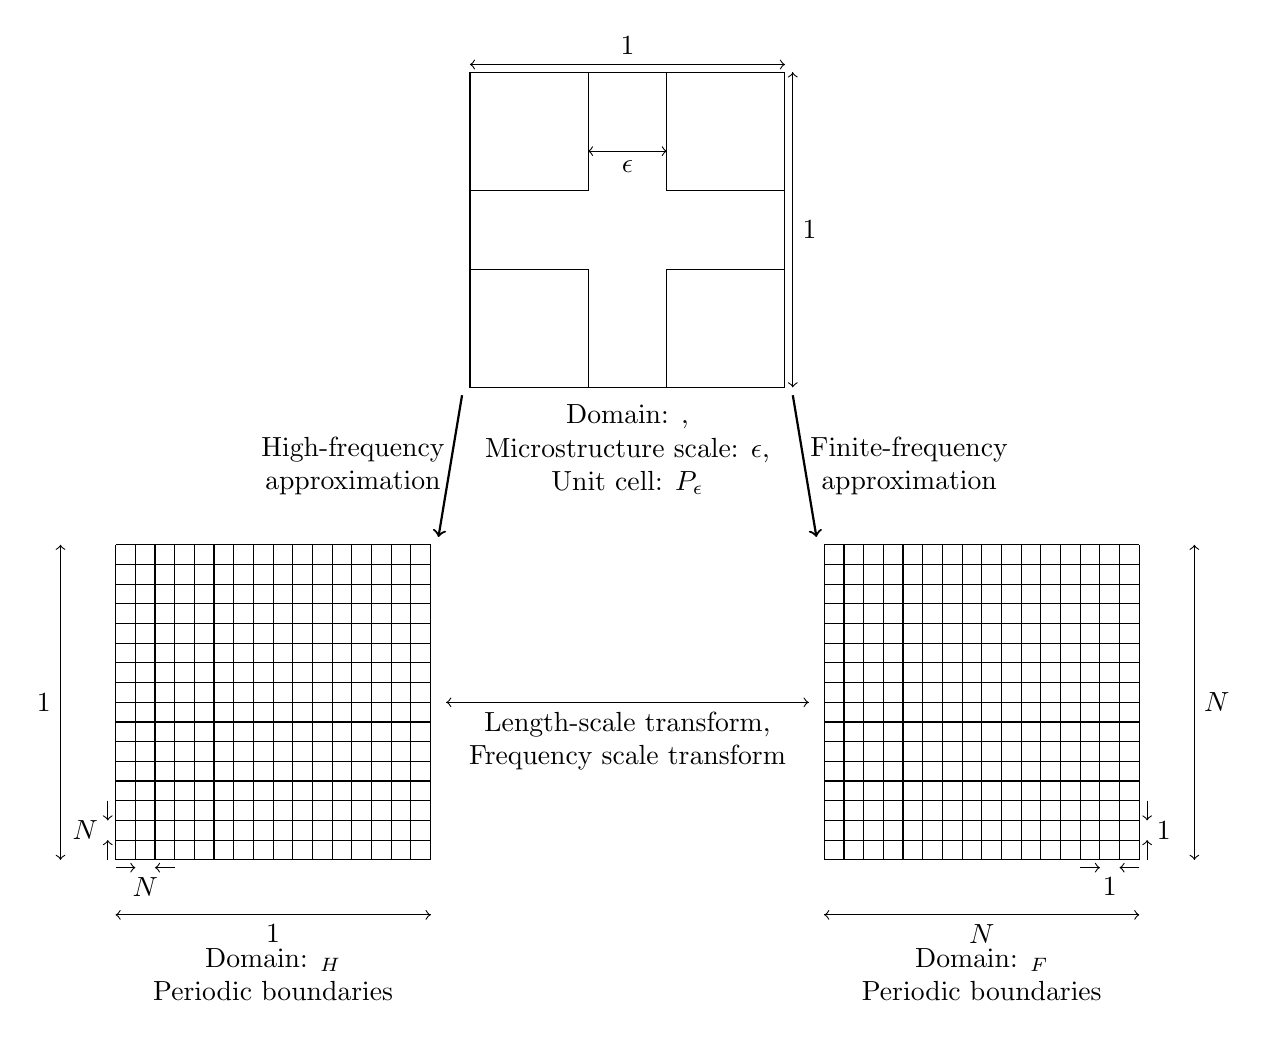
\begin{tikzpicture}
		%Original problem with cubic unit cell, in R^3
		\draw (-2,-2) rectangle (2,2);
		\draw (-0.5,2) -- (-0.5, 0.5) -- (-2,0.5);
		\draw (-2,-0.5) -- (-0.5, -0.5) -- (-0.5, -2);
		\draw (0.5,-2) -- (0.5, -0.5) -- (2,-0.5);
		\draw (2,0.5) -- (0.5,0.5) -- (0.5,2);
		\draw[->] (0.5,1) -- (-0.5,1);
		\draw[->] (-0.5,1) -- (0.5,1);
		\node[anchor=north] at (0,1) {$\epsilon$};
		\draw[->] (-2,2.1) -- (2,2.1);
		\draw[->] (2,2.1) -- (-2,2.1);
		\node[anchor=south] at (0,2.1) {$1$};
		\draw[->] (2.1,-2) -- (2.1,2);
		\draw[->] (2.1,2) -- (2.1,-2);
		\node[anchor=west] at (2.1,0) {$1$};
		\node[anchor=north, align=center] at (0,-2.1) {Domain: $\homDomain$, \\ Microstructure scale: $\epsilon$, \\ Unit cell: $P_{\epsilon}$};
%		\pic {UnitCellCross};
		%Arrow to high frequency approximation
		\draw[thick, ->] (-2.1,-2.1) -- (-2.4,-3.9);
		\node[anchor=east, align=center] at (-2.2, -3.0) {High-frequency \\ approximation};
		%Arrow to low frequency approximation
		\draw[thick, ->] (2.1,-2.1) -- (2.4, -3.9);
		\node[anchor=west, align=center] at (2.2, -3.0) {Finite-frequency \\ approximation};
		%High-frequency approximation setup
		\draw[step=0.25] (-6.5,-8.0) grid (-2.5,-4.0);
		\draw[->] (-7.2,-8.0) -- (-7.2,-4.0);
		\draw[->] (-7.2,-4.0) -- (-7.2,-8.0);
		\node[anchor=east] at (-7.2,-6.0) {$1$};
		\draw[->] (-6.5,-8.7) -- (-2.5,-8.7);
		\draw[->] (-2.5,-8.7) -- (-6.5,-8.7);
		\node[anchor=north] at (-4.5,-8.7) {$1$};
		\draw[->] (-6.6,-8.0) -- (-6.6,-7.75);
		\draw[->] (-6.6,-7.25) -- (-6.6,-7.5);
		\node[anchor=east] at (-6.6,-7.625) {$\recip{N}$};
		\draw[->] (-6.5,-8.1) -- (-6.25,-8.1);
		\draw[->] (-5.75,-8.1) -- (-6.0,-8.1);
		\node[anchor=north] at (-6.125,-8.1) {$\recip{N}$};
		\node[anchor=north, align=center] at (-4.5,-9.0) {Domain: $\homDomain_{H}$ \\ Periodic boundaries};
		%Low-frequency approximation setup
		\draw[step=0.25] (2.5,-8.0) grid (6.5,-4.0);
		\draw (2.5,-8.0) -- (2.5,-4.0); %missing from grid for some reason
		\draw[->] (7.2,-8.0) -- (7.2,-4.0);
		\draw[->] (7.2,-4.0) -- (7.2,-8.0);
		\node[anchor=west] at (7.2,-6.0) {$N$};
		\draw[->] (6.5,-8.7) -- (2.5,-8.7);
		\draw[->] (2.5,-8.7) -- (6.5,-8.7);
		\node[anchor=north] at (4.5,-8.7) {$N$};
		\draw[->] (6.6,-8.0) -- (6.6,-7.75);
		\draw[->] (6.6,-7.25) -- (6.6,-7.5);
		\node[anchor=west] at (6.6,-7.625) {$1$};
		\draw[->] (6.5,-8.1) -- (6.25,-8.1);
		\draw[->] (5.75,-8.1) -- (6.0,-8.1);
		\node[anchor=north] at (6.125,-8.1) {$1$};
		\node[anchor=north, align=center] at (4.5,-9.0) {Domain: $\homDomain_{F}$ \\ Periodic boundaries};
		%Length-scale arrow
		\draw[->] (-2.3,-6.0) -- (2.3,-6.0);
		\draw[->] (2.3,-6.0) -- (-2.3,-6.0);
		\node[anchor=north, align=center] at (0.0, -6.0) {Length-scale transform, \\ Frequency scale transform};
	\end{tikzpicture}
	\caption{Illustration of the original, finite-frequency and high-frequency problems; their domains, and their relation to each other. This represents a 2D-system with period cell the unit square (the 2-dimensional analogue of the text). \label{fig:AsymRegimeDiagram}}
\end{figure} \newline

A note on convention at this point - throughout this report we will refer to $\omega$ as \say{eigenfrequencies}, and $\omega^{2}$ as the eigenvalues.
This is because a large portion of our analysis will focus on determining $\omega$, rather than $\omega^{2}$ and so provide a clear naming convention to make this distinction.
However we will often refer to the spectrum of some operator in terms of the eigenfrequencies $\omega$, rather than the eigenvalues $\omega^{2}$ --- when this is done we refer to the spectrum composed of the eigenvalues $\omega^{2}$ which correspond to the eigenfrequencies $\omega$.
Lastly we remark that the choice of finite-frequency or baseline approximation determines the language used to describe the other frequency approximation, as these are all relative.
We could have chosen (perfectly reasonably) to call the problem in $\homDomain_{H}$ the finite-frequency approximation, in which case the problem in $\homDomain_{F}$ would be called a low-frequency approximation. 
In this report we shall be working in the former case, that is with $\homDomain_{F}$ labelled the finite-frequency problem. \newline


\section{Asymptotic Regimes, Thin Structure Problems and Band Gap Spectra} \label{sec:AsymRegimes}
Having chosen a frequency approximation to work with (and adopting the setup from the previous section), the two length scales $N, \epsilon$ now present us with various asymptotic limits to explore, which can be used to inform us about the spectrum of the original problem.
The end goal of analysing the \say{effective problem} is to provide a means of estimating\footnote{Formally it is necessary to qualify this notion of estimate and associated convergence, as we are considering a limit of a sequence of sets and so the meaning of convergence is not obvious. One may interpret this convergence in the Hausdorff sense, for example.} the spectrum of the original problem by way of understanding a simpler problem, or alternatively to obtain a problem in which an analytic approach is feasible.
Let us denote the periodic full-space domain with microstructure-length scale $\epsilon$ as $\homDomain_{\epsilon}$; the case $\epsilon=0$ is regarded as the singular-structure domain and so has associated embedded graph $\graph$.
Introducing the domain-length scale $N$ gives us set of finite-frequency domains $\homDomain_{\epsilon, N}$ on which we want to find the spectrum, $\bracs{\sigma_{\epsilon, N}}$, of the appropriate operator $\graphOp_{\epsilon, N}$ on $u\in\lp{2}{\homDomain_{\epsilon, N}}$.
We denote this eigenvalue problem by $\mathcal{P}_{\epsilon, N}$.
Each of the limits $N\rightarrow\infty$ and $\epsilon\rightarrow0$ then provides us with a sequence of problems $\bracs{\mathcal{P}_{\epsilon, N}}$ and an associated sequence of spectra $\bracs{\sigma_{\epsilon, N}}$ which converges to the spectrum of an operator that acts on functions in the full-space.
Taking $\epsilon=\epsilon^{*}>0$ as fixed for example, and sending $N\rightarrow\infty$ provides a sequence of problems whose spectra $\sigma_{\epsilon^{*}, N}\rightarrow(0,\infty)$ as $N\rightarrow\infty$, which is the spectrum of a periodic thin-structure medium occupying the whole of $\reals^{d}$. 
One can obtain approximations to each $\sigma_{\epsilon^{*}, N}$ numerically, using e.g. the finite element method which we do in \cref{Homogenisation}). \newline

Other limits involving $\epsilon\rightarrow0$ offer more variety in the resulting effective problems.
In these limits the microstructure becomes singular structure, and the periodic cell can be represented by a graph (hence these problems are referred to as singular structure problems).
The edges and vertices of this graph are determined by the geometry of the unit cell; but colloquially the edges represent the \say{zero-thickness} microstructure, and the vertices \say{junctions} or connections - this is illustrated in \fref{StrucToGraphExample}.
\begin{figure}[b!]
	\centering
	\begin{tikzpicture}
		%microstructure problem
		\draw (-4,-2) rectangle (0,2);
		\draw (-2.5,2) -- (-2.5, 0.5) -- (-4,0.5);
		\draw (-4,-0.5) -- (-2.5, -0.5) -- (-2.5, -2);
		\draw (-1.5,-2) -- (-1.5, -0.5) -- (0,-0.5);
		\draw (0,0.5) -- (-1.5,0.5) -- (-1.5,2);
		%red stuff to mark connections or junctions
		\draw[red] (-2,2) circle (0.5);
		\draw[red] (-2,-2) circle (0.5);
		\draw[red] (-4,0) circle (0.5);
		\draw[red] (0,0) circle (0.5);
		\draw[red] (-2,0) circle (0.707);
		%arrow and eps-->0 limit
		\draw[->, thick] (0.5,0) -- (1.7,0);
		\node[anchor=south] at (1.1,0) {$\epsilon\rightarrow0$};
		%graph problem
		\draw (2,0) -- (6,0);
		\draw (4,-2) -- (4,2); %graph lines done
		\filldraw[red] (2,0) circle (2pt);% node[anchor=north west] {$n_{1}$};
		\filldraw[red] (6,0) circle (2pt);
		\filldraw[red] (4,-2) circle (2pt);
		\filldraw[red] (4,2) circle (2pt);
		\filldraw[red] (4,0) circle (2pt); %nodes done
	\end{tikzpicture}
	\caption{Illustration of a graph problem obtained by letting $\epsilon\rightarrow0$, the mcirostructure on the left is represented by the graph on the right. Red circles represent regions where connections and junctions in the microstructure occur, which become nodes in the graph representation.  \label{fig:StrucToGraphExample}}
\end{figure}
The effective problem is a singular-structure problem and so the theory discussed in \sref{GraphPrelims} is applicable.
The domain is a periodic graph $\graph = \bracs{V, E}$ on which we are seeking the spectrum of the operator $\graphOp_{0, N}$.
The appropriate boundary conditions to apply at the vertices depend on the scaling of the so-called edge-\say{volume} $\eVol$ and vertex-\say{volume}\footnote{To illustrate what is meant by vertex- and edge-volume we can use the 2-dimensional examples in \fref{AsymRegimeDiagram} and \fref{StrucToGraphExample}: each edge has $\eVol$ equal to the volume of the arms of the cross, whose width is $\epsilon$ and so $\eVol\propto\epsilon$. The vertices (at the centre of the cross and the edges) have radius proportional to $\epsilon$, and so $\vVol\propto\epsilon^{2}$ - note that if we were in 3-dimensions the volumes would scale at different rates.} $\vVol$ \cite{exner2005convergence} in $\homDomain$.
The relative scaling of $\vVol$ and $\eVol$ determines the appropriate boundary conditions at the interior vertices of the graph, which ensure that the spectrum of the singular structure problem coincides with the limit $\sigma_{\epsilon, N^{*}}$ as $\epsilon\rightarrow0$.
To describe each case, we adopt the language of \cite{exner2005convergence}:
\begin{itemize}
	\item \underline{Fast-Decaying $\vVol$:} If $\vVol$ decays significantly faster than $\eVol$ then at the interior vertices we impose continuity of the solution (coming from each of the edges into the vertex) and a classical Kirchhoff condition. 
	A classical Kirchhoff condition imposes that the sum of the derivatives\footnote{Strictly, this sum may also be weighted if the setup of the original problem is correct. 
	However for our purposes this is unnecessary.} of the edge solutions into the vertex (signed according to direction into or out of the vertex) be equal to 0:
	\begin{align*}
		\sum_{e_{j}\in E \text{ connects to } v_{k}} \mathrm{dir}\bracs{u_{j}}u_{j}^{\prime}\bracs{v_{k}} &= 0
	\end{align*}
	where $\mathrm{dir}\bracs{u_{j}}$ stands-in for effect of the directing the derivatives into $v_{k}$.
	\item \underline{Slow-Decaying $\vVol$:} If $\vVol$ decays slower than $\eVol$, the edges are essentially independent from the vertices and the structure effectively \say{breaks down}. 
	We obtain a Dirichlet problem on each edge-interval and vertex-domain, and the resulting spectrum is the union of the spectra of the decoupled problems. 
	This is referred to as \say{Dirichlet decoupling}.
	\item \underline{Boarderline Case:} If $\vVol$ decays at the same rate as $\eVol$, then we obtain conditions of continuity and non-classical Kirchhoff conditions at the interior vertices.
	These non-classical conditions involve the spectral parameter $\omega^{2}$, and have the form
	\begin{align*}
		\sum_{e_{j}\in E \text{ connects to } v_{k}} \mathrm{dir}\bracs{u_{j}}u_{j}^{\prime}\bracs{v_{k}} &= \omega^{2}u\bracs{v_{k}}.
	\end{align*}
	The value of the solution $u\bracs{v_{k}}$ exists due to the condition of continuity that is applied at each interior vertex.
	This non-classical Kirchhoff condition can give rise to \say{band-gap} phenomena, discussed shortly.
\end{itemize}
The sequence of problems $\mathcal{P}_{0, N}$ leads us (as $N\rightarrow\infty$) to a periodic singular structure in the whole of $\reals^{d}$, each spectrum $\sigma_{0, N}$ being a sequence of points on the positive real axis.
These spectra \say{fill up} the positive real axis, producing a spectrum which is a union of intervals in $\bracs{0,\infty}$ and which coincides with the spectrum of a periodic singular-structure problem on the whole of $\reals^{d}$ \cite{exner2005convergence}, \cite{kuchment2001convergence}. 
This raises the concept of a band-gap spectrum, a spectrum which can be represented as a (potentially infinite) union of (disjoint) intervals in the positive real axis, but which does not fill the entirety of $\bracs{0,\infty}$. \newline

One can take the limits $N\rightarrow\infty$ and $\epsilon\rightarrow0$ simultaneously, and in such a way that there exists $N\epsilon^{\alpha}\rightarrow\gamma\in(0,\infty)$ (for some $\alpha, \gamma\in\bracs{0,\infty}$).
The importance of this double limit; besides mathematical curiosity in the properties of the result, is that certain materials may be poorly approximated in the other regimes - and photonic crystals fall into this category.
The resulting limit of the spectra $\sigma_{\epsilon, N}$ is then determined by a singular-structure problem, posed in the whole of $\reals^{d}$, with period cell of side 1 and with vertex boundary conditions determined by the vetex- and edge-volume scaling.
Crucially however, this problem does not represent a periodic singular-structure in the whole of $\reals^{d}$, but rather the original thin-structure problem posed in $\homDomain$.
This provides us with a method of determining the spectrum of thin-structure problems by analysis of thin-structure problems; such problems may be more open to mathematical analysis (which we will demonstrate with the examples in \cref{Graphs}) and also bypass the computational complexities of numerical solvers for problems in multiple dimensions.
This also means that certain periodic, thin-structure materials may have spectra composed of sub-intervals of $\bracs{0,\infty}$, separated by gaps of increasing length (see \sref{Graph2DNonClassicalKirchhoff}).
This idea will be central to our application of the preceding theory to PCFs as the band gap spectrum determines which frequencies of light can (or cannot) propagate in the microstructure.
If the remainder of the domain is interpreted as vacuum (or any dielectric material in the event of a solid-core fibre) then the band gaps determine the frequencies at which the fibre can be used to transmit information, we will develop this further in \cref{WorkDirection}.

\section{Report Outline}
This report intends to demonstrate how the mathematical concepts that we introduced above can assist the development of PCFs.
\Cref{Graphs} aims to demonstrate the theory introduced in \sref{AsymRegimes} by means of explicit examples. 
These examples will focus on the scalar-divergence equation $-\laplacian u=\omega^{2}u$ on a suitable periodic domain $\homDomain\subset\reals^{2}$ with microstructure in each unit cell.
It will explicitly determine the spectrum of the problem in the fast-decaying vertex volume case, demonstrating that the effective problem represents a homogenised medium.
Additionally there will be a presentation of a problem in the borderline case (of vertex scaling) which will demonstrate the concepts of spectral band gaps, and provide some analysis which proves that this particular spectrum is composed of unions of sub-intervals of the positive real axis.
\Cref{Homogenisation} will use numerical techniques (based around the Finite Element Method) to analyse the spectra of a sequence of thin structure problems in the limit $N\rightarrow\infty$, $\epsilon\rightarrow0$ with $N\epsilon^{\alpha}\rightarrow\gamma\in(0,\infty), \alpha>0$.
The purpose of this section will be to demonstrate the technicalities of numerical approaches to this problem, to link up with the demonstrations of \cref{Graphs}, and to reinforce the earlier claim of the spectrum of the effective problem being the limit of the sequence of spectra $\sigma_{\epsilon, N}$.
The report will conclude with \cref{WorkDirection}, which will develop the ideas presented thus far in the context of electromagnetics.
This will include how to physically interpret (and setup) the domains that problems are posed in; a discussion of how to adapt the previous methods to suit the more complex system of Maxwell equations, how such a model would fit into the broader set of existing models for PCFs, and speculate on further generalisations that can be made to the model and how these might be implemented.
This will culminate in a summary of the ideas that have been presented and a proposal for studying PCFs using the theory and methods discussed in the report.